\documentclass[12pt, authoryear]{elsarticle}
\makeatletter
\def\ps@pprintTitle{%
	\let\@oddhead\@empty
	\let\@evenhead\@empty
	\def\@oddfoot{}%
	\let\@evenfoot\@oddfoot}
\makeatother
%\usepackage{lmodern}
% My spacing
\usepackage{setspace}
\setstretch{1.5}
\usepackage{multirow}
%\DeclareMathSizes{12}{14}{10}{10}
\usepackage[margin=2.5cm]{geometry}    % How to set margins - optimized for 2.5cm      
\usepackage[capposition=top]{floatrow}

% See geometry.pdf to learn the layout options. There are lots.
\geometry{a4paper}                   			% ... or a4paper or a5paper or ... 
\usepackage{enumitem}
\usepackage{mathtools}
%\geometry{landscape}                		% Activate for rotated page geometry
\usepackage[parfill]{parskip}    			% Activate to begin paragraphs with an empty line rather than an indent
\usepackage{graphicx}						% Use pdf, png, jpg, or eps§ with pdflatex; use eps in DVI mode
% TeX will automatically convert eps --> pdf in pdflatex	
\usepackage{flafter}			
\usepackage{setspace}
%\linespread{1.5}
\usepackage[font={}]{caption}
\usepackage[bottom]{footmisc}
\usepackage[capposition=top]{floatrow}   %figure notes
\usepackage{lscape}
%math packages 
\usepackage{amssymb}
\usepackage{fancyhdr}
\usepackage{graphicx,epsf,subfigure}
\usepackage{pstricks,pst-node,psfrag}
\usepackage{amsthm,amssymb,amsmath}
\usepackage{amsmath,bm}

%mathnotes
\newcommand{\bbeta}{\mbox{\boldmath $\beta$}}
\newcommand{\beps}{\mbox{\boldmath $\epsilon$}}
\newcommand{\bX}{\mbox{\boldmath $X$}}
\newcommand{\bY}{\mbox{\boldmath $Y$}}
\newcommand{\bI}{\mbox{\boldmath $I$}}
\newcommand{\N}{\mathcal{N}}
\newcommand{\x}{\textsc{\textbf{x}}}
\newcommand{\xx}{\textsc{x}}
\definecolor{aurometalsaurus}{rgb}{0.43, 0.5, 0.5}
%add figure 
\DeclareGraphicsRule{.tif}{png}{.png}{`convert #1 `dirname #1`/`basename #1 .tif`.png}
\usepackage{rotating}
\usepackage{pdflscape}
\usepackage{hyperref}
\usepackage[round]{natbib}
	\definecolor{ashgrey}{rgb}{0.7, 0.75, 0.71}
\usepackage{soul}
 \usepackage{animate}

\def\bibsection{\section{References}} %%% Make "References" appear before bibliography
\usepackage{longtable}
\usepackage{hyperref}
\usepackage{tablefootnote}
\usepackage{lscape} 
\usepackage{animate}

\renewcommand{\contentsname}{Table of Contents} % change name from Contents to Table of Contents

\usepackage{titlesec}

\setcounter{secnumdepth}{4}

%_______________________________________________________________________________________________________%
%_______________________________________________________________________________________________________%
%\usepackage[table]{xcolor}% http://ctan.org/pkg/xcolor
%\usepackage{graphicx,multirow}
\usepackage{xcolor,colortbl}
\usepackage{xcolor}
%\usepackage{graphicx,multirow}
\usepackage[capposition=top]{floatrow}
\setcounter{secnumdepth}{4}
\usepackage{tikz}
\begin{document}

\begin{frontmatter}  %

\title{ GRADIENT DESCENT VS NEWTON'S METHOD \\ \vspace{0.5cm} \large 
 THE ALGORITHMIC SHOWDOWN
}

\author[Add1]{Reid Falconer}
\ead{reid.falconer@bracelonagse.eu}

\address[Add1]{Barcelona Graduate School of Economics, Barcelona, Spain}
%\address[Add2]{Some other Institution, Cape Town, South Africa}

%\cortext[cor]{Corresponding author: Nico Katzke}

%\begin{abstract}
%\small{
%Abstract to be written here. 
%}
%\end{abstract}

%\vspace{1cm}

\begin{keyword}
\footnotesize{
Line Search \sep  Gradient Descent \sep Newton's Method \\ \vspace{0.3cm}
%\textit{JEL classification} L250 \sep L100
}
\end{keyword}
\vspace{0.5cm}
\end{frontmatter}

\headsep 25pt % So that header does not go over title

\section{Outline}

Line search methods are used widely for numerical optimisation. This project seeks to determine how two line search methods, namely gradient descent and Newton's method, perform relative to each other and to further assess the differences in the execution of first order and second order optimisation algorithms.

Let $\boldsymbol { x } \in \mathbb { R } ^ { n }$ and consider the function
\begin{equation}
\begin{aligned}
f ( \boldsymbol{ x} ) = \frac { 1 } { 2 } ( \boldsymbol{ x}  - \boldsymbol{ m}  ) ^ { \top } A ( \boldsymbol{ x}  - \boldsymbol{ m}  ) - \sum _ { i = 1 } ^ { n } \log \left( x _ { i } ^ { 2 } \right)
\label{function}
\end{aligned}
\end{equation}
where $\boldsymbol { m } \in \mathbb { R } ^ { \mathbf { n } }$ is a fixed vector and $A \in \mathbb { S } _ { t + } ^ { n }$ is a fixed positive definite matrix.

We will primarily focus on the two-dimensional case $(n = 2)$. Where $\boldsymbol{m}$ is fixed at $\boldsymbol{m} = (0.5, 0)$ and we will study the convergence of the two algorithmic methods mentioned above depending on $\rho \in ( - 1,1 )$ in
\[
A = \left[ \begin{array} { l l } { 1 } & { \rho } \\ { \rho } & { 1 } \end{array} \right]
\]

More specifically, in this analysis we will implement the \textit{gradient descent} and \textit{newton's method} for the problem of minimising function (\ref{function}).  Furthermore, we will also explore how the performance of the two algorithms scales with $n$ equal to 50, 100, 200, 500 and 1000.

\subsection{Gradient Descent}

Gradient descent is a simple method for numerical optimisation, similar to some of the methods you can use with the `optim()' function in R, but here we will explicitly program it. It is an alternative to analytical solutions that cannot always be employed. For example, data might be too big, or matrix inversion may be too costly.

More precisely, gradient descent is an iterative method that starts with an initial guess ($\boldsymbol{x} ^ { ( 0) }$) and updates the parameters in each iteration by the amount of the gradient multiplied by a learning rate, $\alpha_t$
\begin{equation}
\begin{aligned}
\boldsymbol{x} ^ { ( t + 1 ) } = \boldsymbol{x} ^ { ( t ) } - \alpha_{ t } \nabla f \left( \boldsymbol{x} ^ { ( t ) } \right)
\label{gd_update}
\end{aligned}
\end{equation}

where $\boldsymbol{x}$ is a vector of parameters and $\bigtriangledown f(\boldsymbol{x}^ { ( t ) })$ is the gradient of the objective function $f(\boldsymbol{x})$, that is, a derivative of our objective function with respect to the parameters.  
 
Additionally, given that the learning rate can substantially modify the behaviour of the algorithm (if it is too big the algorithm may not converge), we also implement basic backtracking, where we start with $\alpha_t = 1$ and check whether $ f \left( \boldsymbol{x} ^ { ( t + 1 )} \right) <  f \left(   \boldsymbol{x} ^ { ( t ) } - \alpha_{ t } \nabla f \left( \boldsymbol{x} ^ { ( t ) } \right) \right)  $. If not, $\alpha_t \leftarrow \alpha_t/ 2$ and repeat.


\subsection{Newton's Method}

The Newton-Raphson method, or Newton method, is also a powerful technique for solving equations numerically. It is very similar to gradient descent however, Newton's method requires the function  $f(\boldsymbol{x})$ to be twice differentiable. This is because Newton's method updates the parameters in each iteration by the amount of the gradient ($ \nabla f ( { \boldsymbol { x }^ {( t)}})$) multiplied by the inverse of the Hessian matrix ( $( \nabla^{ 2 }f( { \boldsymbol { x}^ { ( t ) }})^{-1} $), which is a square matrix of second-order partial derivatives of the function (\ref{function}). 

Intuitively, the Hessian describes the local curvature of the loss function, which allows us to perform a more efficient update. In particular, multiplying by the inverse Hessian leads the optimisation to take more aggressive steps in the directions of shallow curvature and shorter steps in directions of steep curvature. Note, crucially, the absence of any learning rate hyper-parameters in the update formula, which the proponents of these methods cite this as a large advantage over first-order methods. Therefore, 
\begin{equation}
\begin{aligned}
\boldsymbol{x} ^ { ( t + 1 ) } = \boldsymbol{x} ^ { ( t ) } -  (\nabla^{ 2 }f( { \boldsymbol { x}^ { ( t ) }}))^{-1} \nabla f \left( \boldsymbol{x} ^ { ( t ) } \right)
\label{new_update}
\end{aligned}
\end{equation}

However, to make the two algorithms more comparable, we modify Newton's method to include a learning rate,$\gamma_{ t }$, to enable us to implement basic backtracking. Consequently,
\begin{equation}
\begin{aligned}
\boldsymbol{x} ^ { ( t + 1 ) } = \boldsymbol{x} ^ { ( t ) } -   \gamma_{ t } (\nabla^{ 2 }f( { \boldsymbol { x}^ { ( t ) }}))^{-1} \nabla f \left( \boldsymbol{x} ^ { ( t ) } \right)
\label{new_gamma_update}
\end{aligned}
\end{equation}

where we start with $\gamma_t = 1$. We then check whether $ f \left( \boldsymbol{x} ^ { ( t + 1 )} \right) <  f \left(   \boldsymbol{x} ^ { ( t ) } -  \gamma_{ t } (\nabla^{ 2 }f( { \boldsymbol { x}^ { ( t ) }}))^{-1} \nabla f \left( \boldsymbol{x} ^ { ( t ) } \right)\right)  $. If not, $\gamma_t \leftarrow \gamma_t/ 2$ and repeat.

\section{Gradient Descent vs Newton's Method}  \label{sec1}

\subsection{Contour Plots}
We begin the algorithmic showdown by focusing on the two-dimensional case ($n = 2$) where $\boldsymbol{m} = (0.5; 0)$. Firstly, we illustrate the contour plots with the sample paths of both algorithms, while scrolling through $\rho = -0.9$ to $0.9$ in increments of $0.1$.  

The ellipses in Figure \ref{fig:rho} are the contours of the quadratic function (\ref{function}), and the red and blue lines are the trajectories taken by Newton's method and gradient descent respectively, which were both initialised at $\boldsymbol{x} ^ { ( 0) } = [-3.5; 1]^\top $ for every $\rho$. Furthermore, the black circles in the figure (joined by the trajectory lines) mark the successive values of $\boldsymbol{x}$ that the Newtons method and gradient descent go through (i.e. the iterations).

Interestingly, it can be seen that the two algorithms find different local minima for specific values of $\rho$, even when initialised at the same point. Therefore, clearly, the algorithms cannot distinguish between a local minimum and a global minimum since they both approximate the function as a quadratic, which can only have one minimum. Moreover, it appears that Newton's method converges to a local minimum in significantly fewer iterations when compared to gradient descent (this will be confirmed in the next section) although they both take steps of roughly the same length.

\begin{figure}[H]
	\begin{center}
		\animategraphics[autoplay,loop,controls=true,scale=0.15]{0.8}{images/fig_}{1}{19}
		\caption{Gradient Descent vs Newton's Method, contour plots with sample paths, scrolling through $\rho = -0.9 : 0.9$}
		\label{fig:rho}
		\floatfoot{Notes: Starting point initialised at $(-3.5,1)$}
	\end{center}
	\vspace{5mm}
%	\float{\small See \ref{gammaaapp} for static pannels.}
\end{figure}

\subsection{Iterations and Runtime ($n=2$)}

The second part of the showdown involves assessing the average number of iterations\footnote{The average number of iterations are calculated by averaging the number iterations of 500 simulations at every $\rho$} required by each algorithm to converge to a local minimum, while scrolling through $\rho = -0.9$ to $0.9$. Figure \ref{fig:iterations} highlights this result and confirms that Newton's method requires substantially fewer iterations to converge, compared to gradient descent, across all values of $\rho$. Gradient descent requires 89 and 77 iterations on average at $\rho = -0.9$ and $\rho = 0.9$ respectively, and only needs approximately 6 iterations when $\rho = 0$. Conversely, Newton's method needs only 4 iterations , on average, across all values of $\rho$. 

\begin{figure}[H]
	\centering
	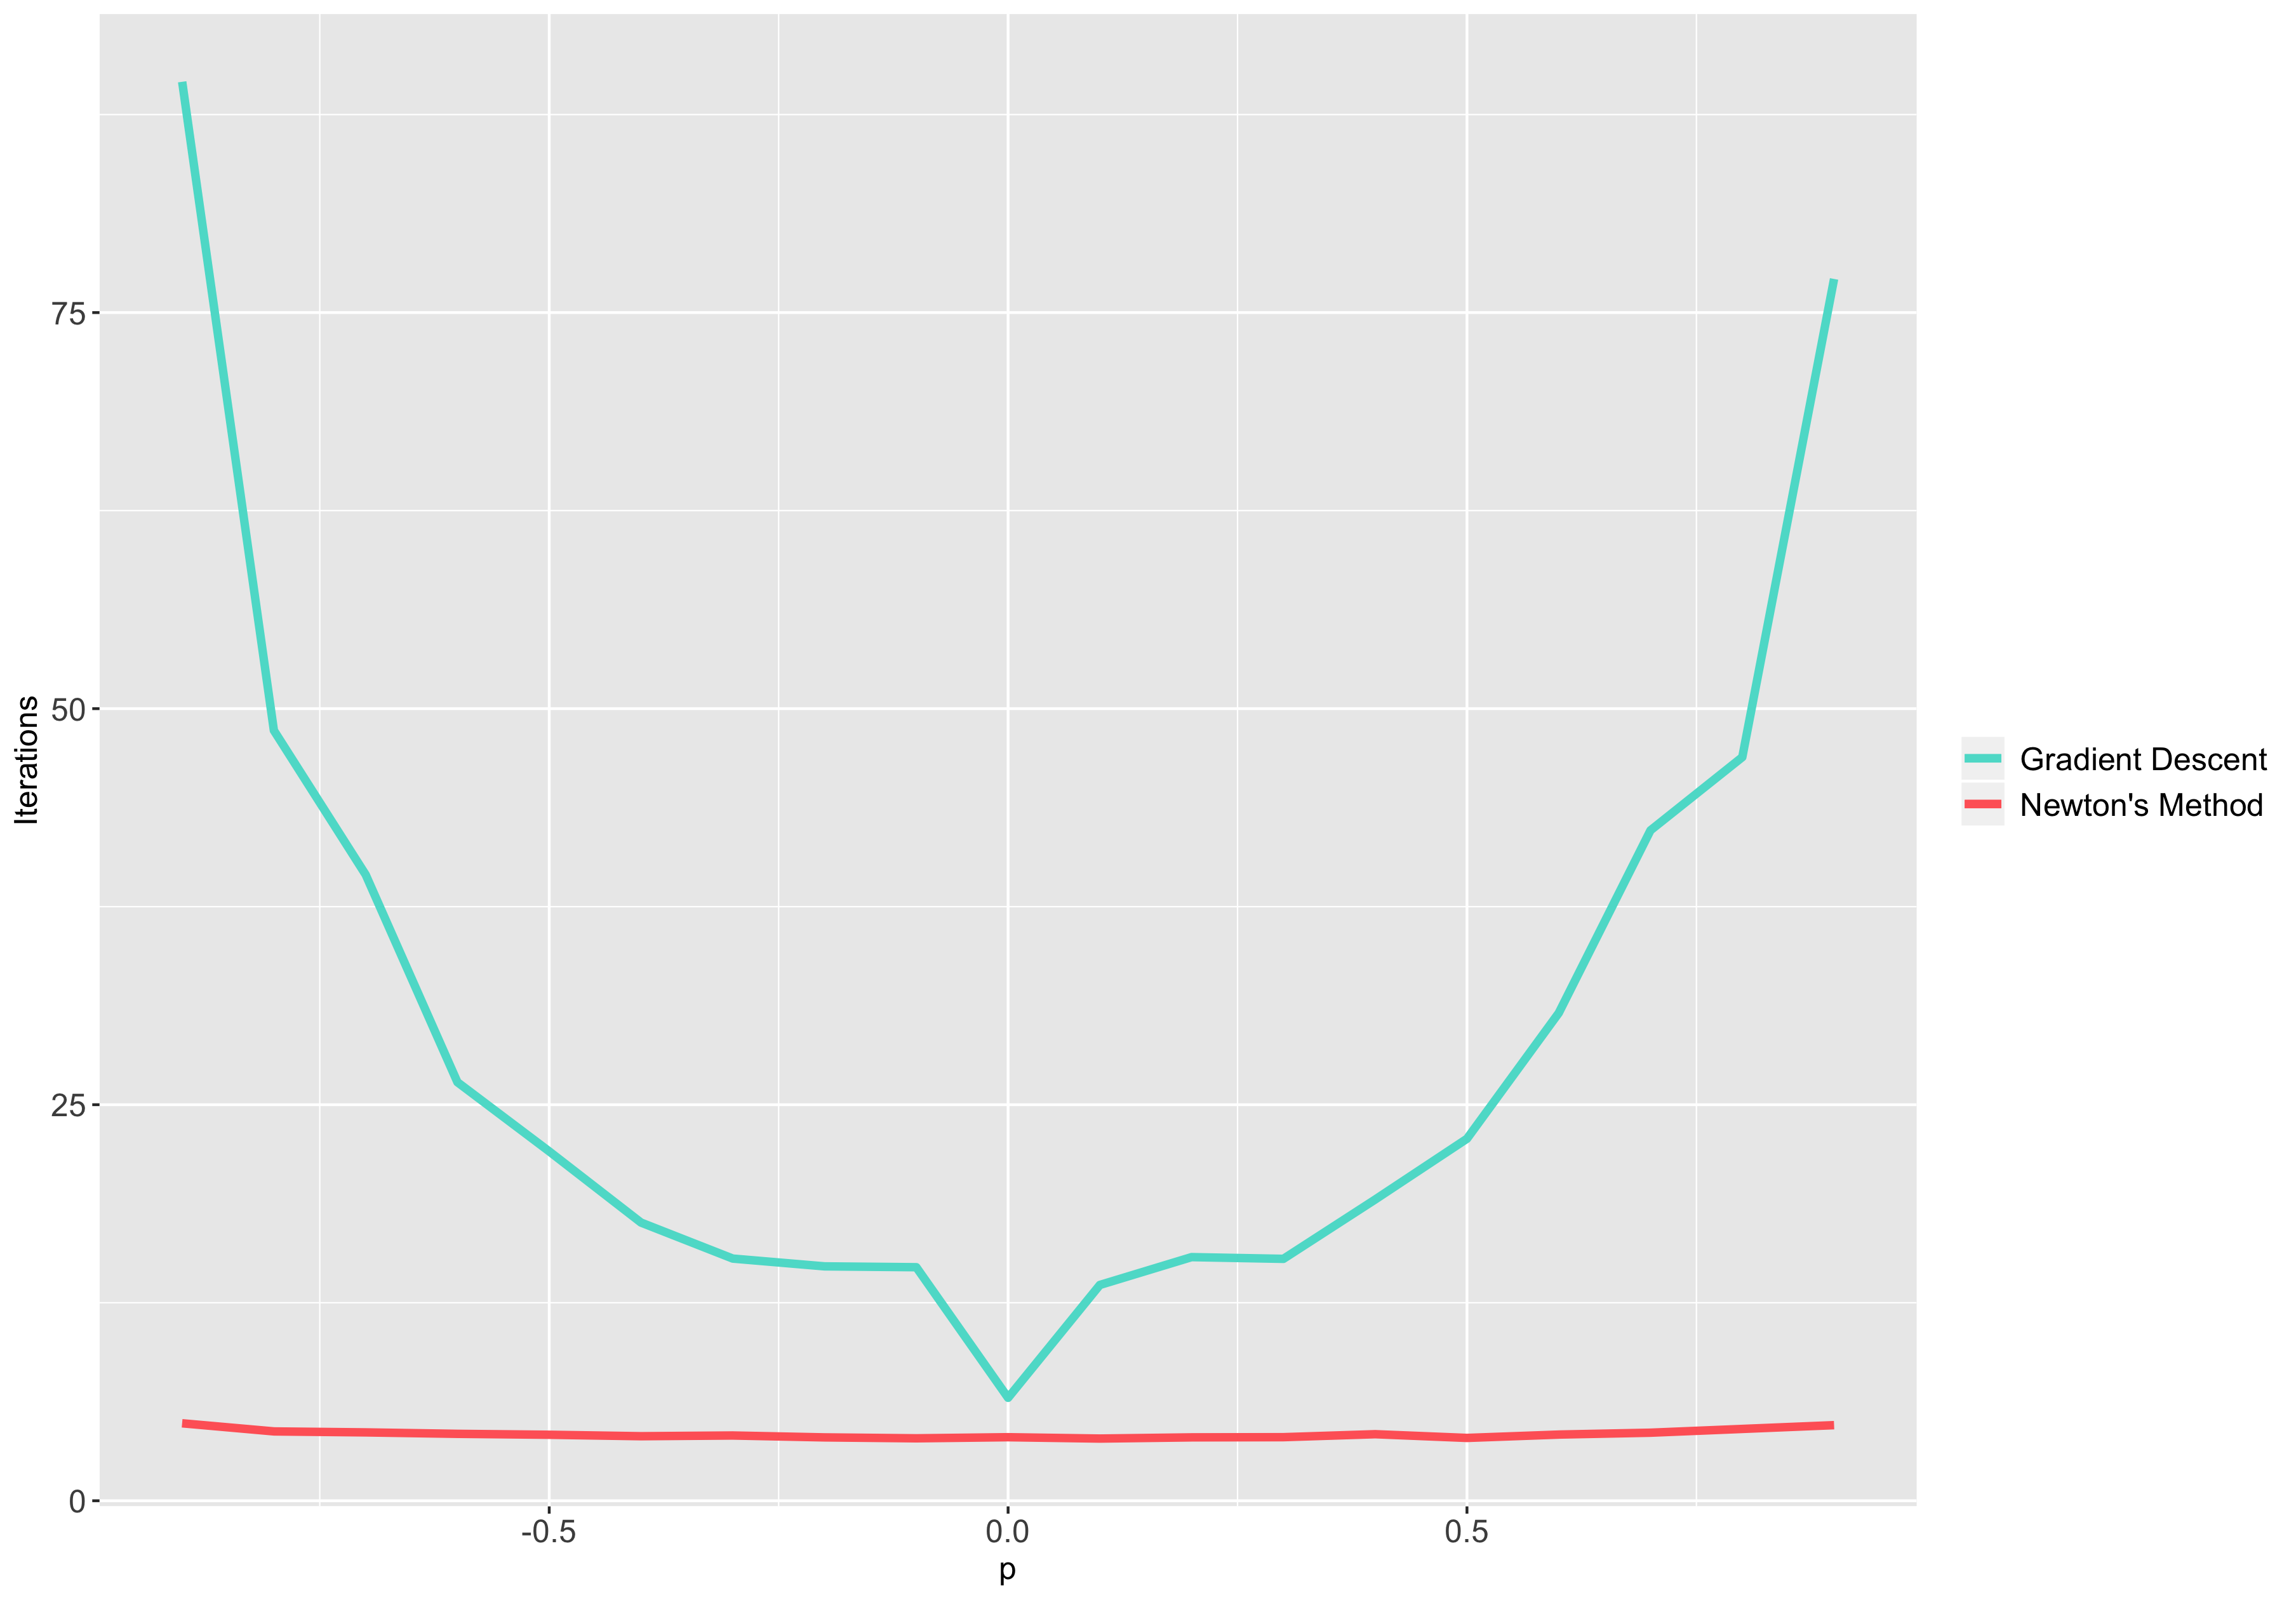
\includegraphics[clip, angle=0, width=13cm]{images/iterations.png}
	\caption{Average number of iterations over $\rho$}
	\label{fig:iterations}
	\floatfoot{Notes: The average number of iterations are calculated by averaging the number iterations of 500 simulations at every $\rho$ }
\end{figure}

Nevertheless, when assessing the average runtime\footnote{The average runtimes are calculated by averaging the runtimes of 500 simulations at every $\rho$}  of the algorithms while scrolling through $\rho = -0.9$ to $0.9$ it can be seen (see Figure \ref{fig:convergence}) that there are no significant differences between the two methods.

\begin{figure}[H]
	\centering
	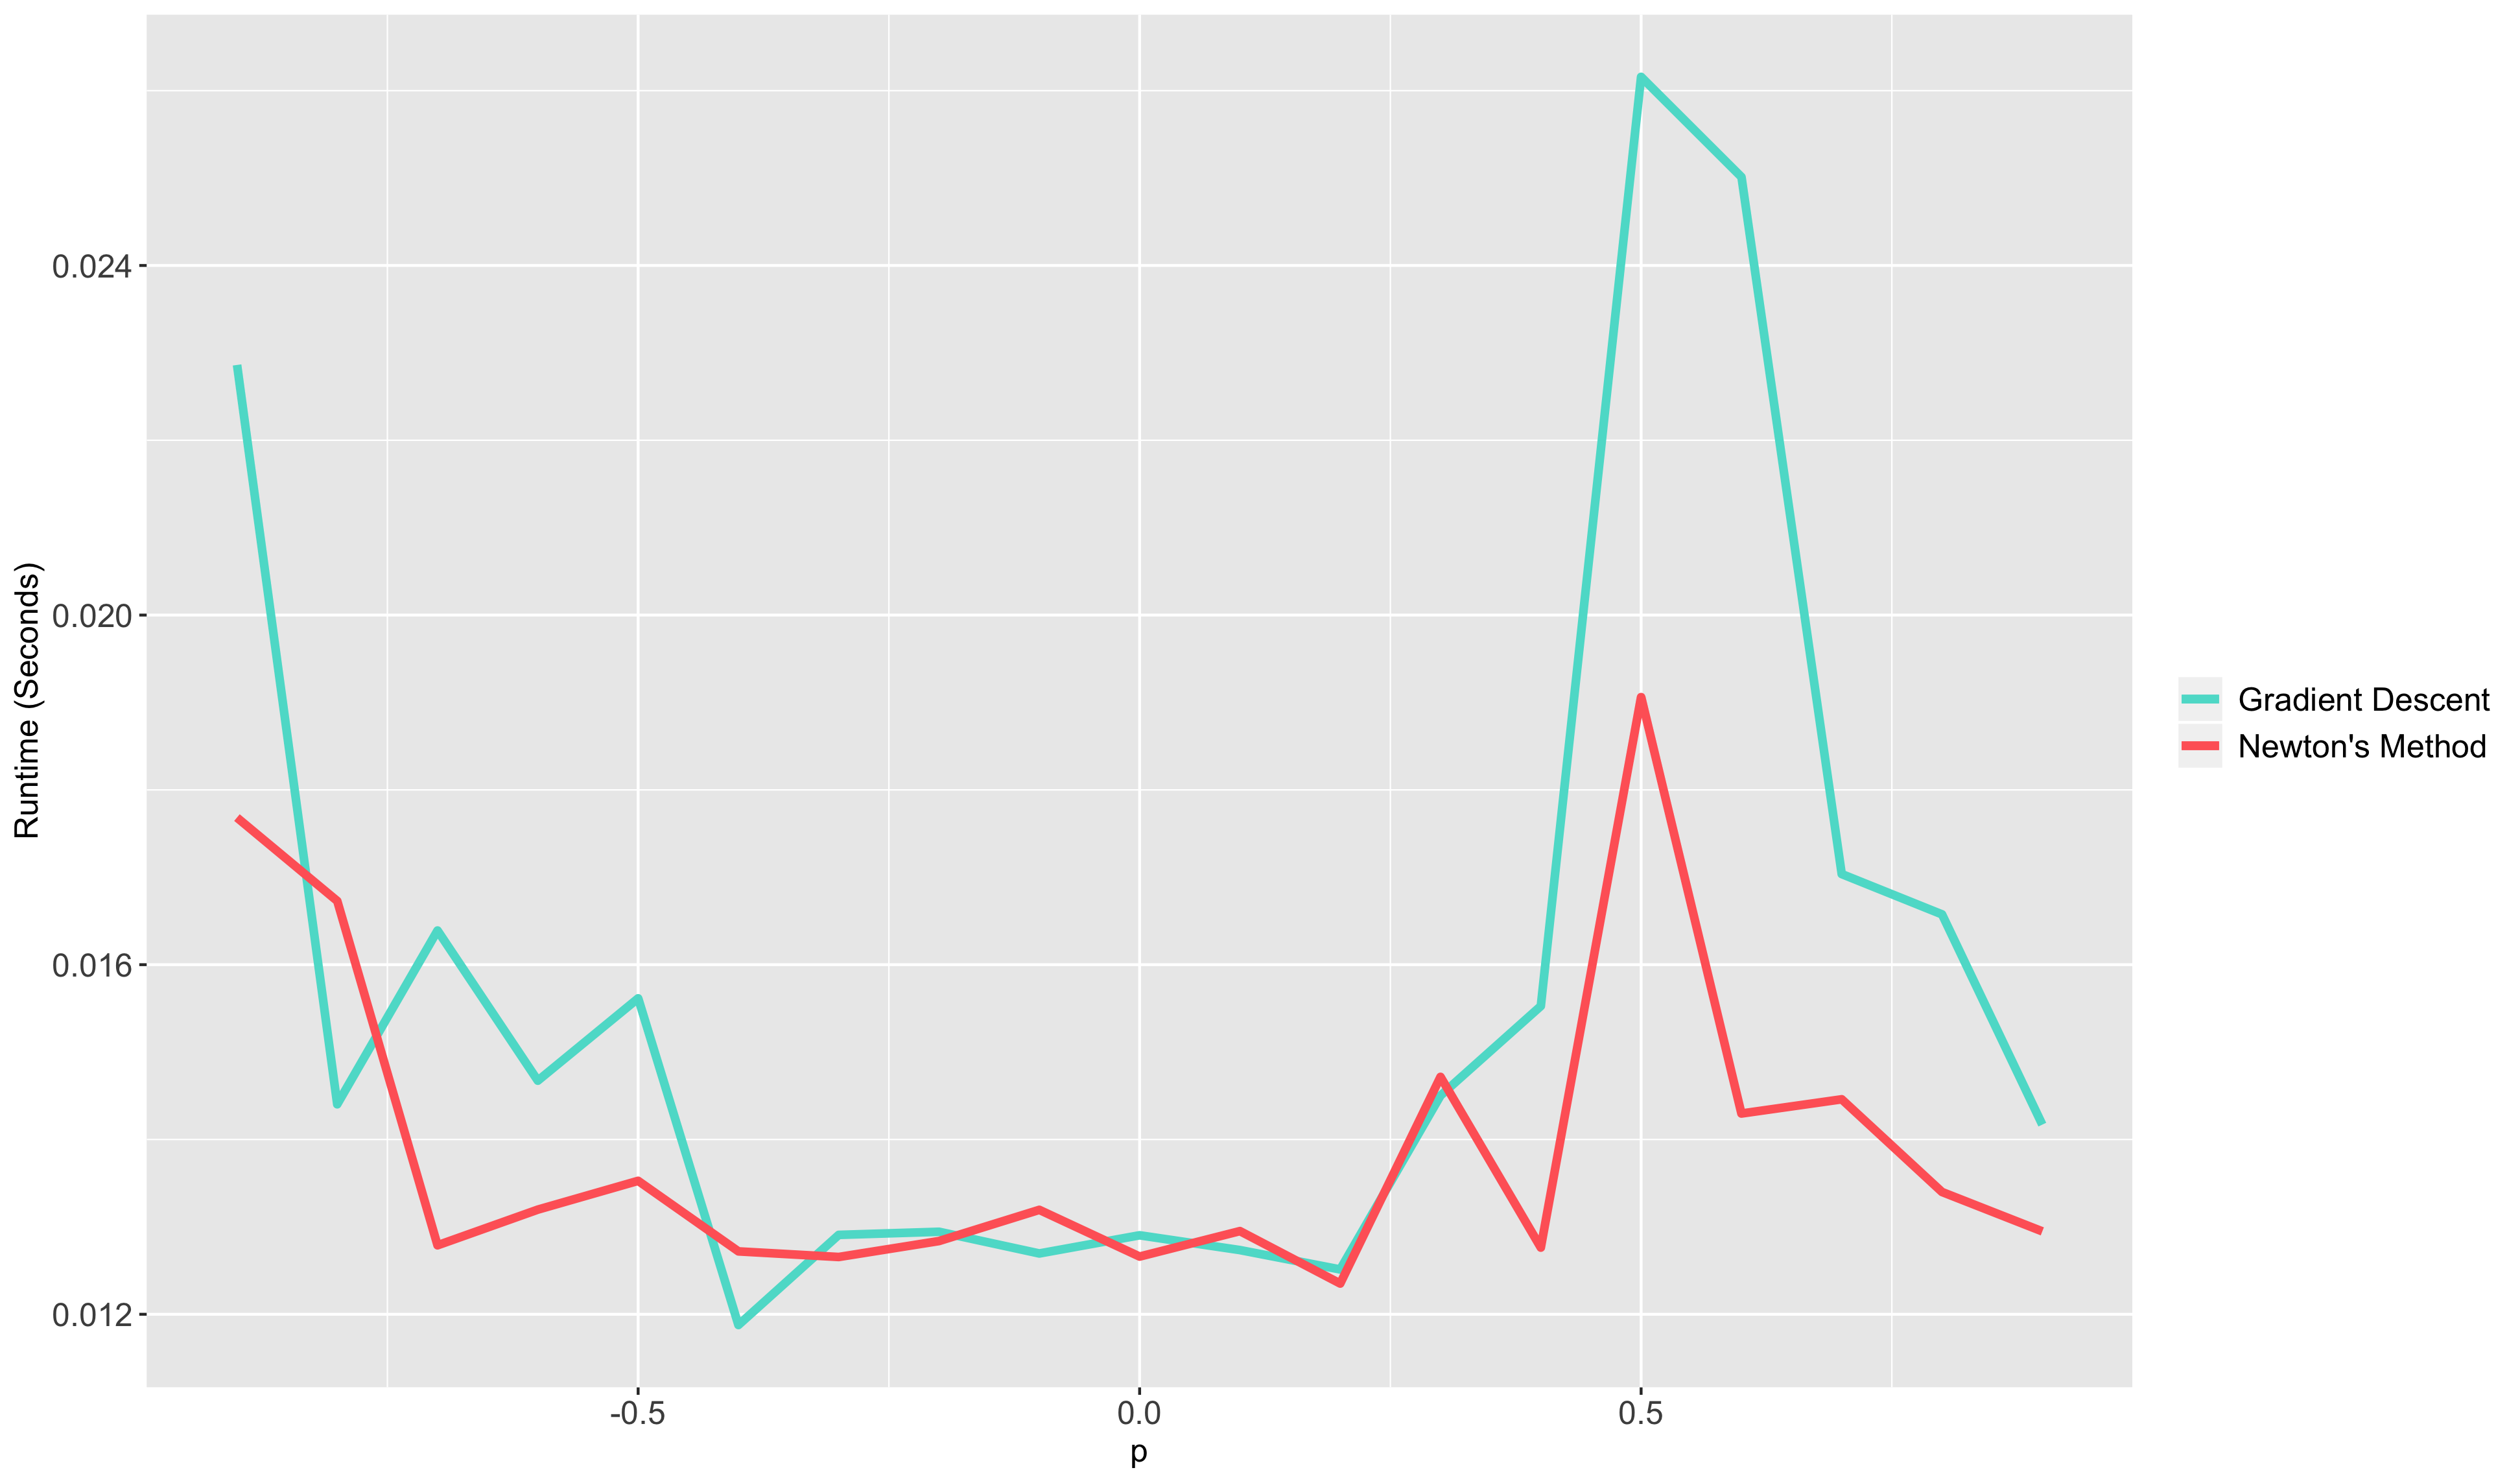
\includegraphics[clip, angle=0, width=13cm]{images/convergence.png}
	\caption{Average runtime (seconds) over $\rho$}
	\label{fig:convergence}
	\floatfoot{Notes: The average runtimes are calculated by averaging the runtimes of 500 simulations at every $\rho$ }
\end{figure}


\section{Higher Dimensions}  \label{sec2}

Optimising functions of this kind has recently become important in Bayesian model selection procedures involving high-dimensional regression problems. In that case, $n$ will be much larger, say 50, 100, 200, 500 or 1000. Therefore, in this part of the showdown, we will choose random values for $\boldsymbol{m}$ and $A$ (see function (\ref{function}))\footnote{Where $\boldsymbol{m}$ is drawn from a uniform distribution $\boldsymbol{m} \in \{-1, 1\})$ with $n$ observations and $A$ is drawn from a normal distribution with a mean equal to $0$ and standard deviation equal to $1$ with $n*n$ observations.} and study (by simulations) how the performance of gradient descent and Newton's method scales with $n$.

\subsection{Iterations and Runtime ($n=50, 100, 200, 500$ and $1000$)}

The final part of this showdown assess the average number of iterations\footnote{The average number of iterations are calculated by averaging the number iterations of 100 simulations for dimensions $n$} and the average runtime\footnote{The average runtimes are computed by averaging the runtimes of 100 simulations for dimensions ($n$)} of the algorithms while scaling $n$.

Figure \ref{fig:dimensions} and Table \ref{dim_table} depict the average number of iterations required by each algorithm to converge to a local minimum, for different dimensions ($n$). Newton's method scales well with $n$, as it only requires between 8 and 13 iterations, on average, across all dimensions to converge. Conversely, gradient descent scales poorly and requires significantly more iterations at every dimension of $n$. Furthermore, unlike Newton's method where the iterations remain fairly constant over $n$, gradient descent requires more iterations as $n$ increases.  

\begin{figure}[H]
	\centering
	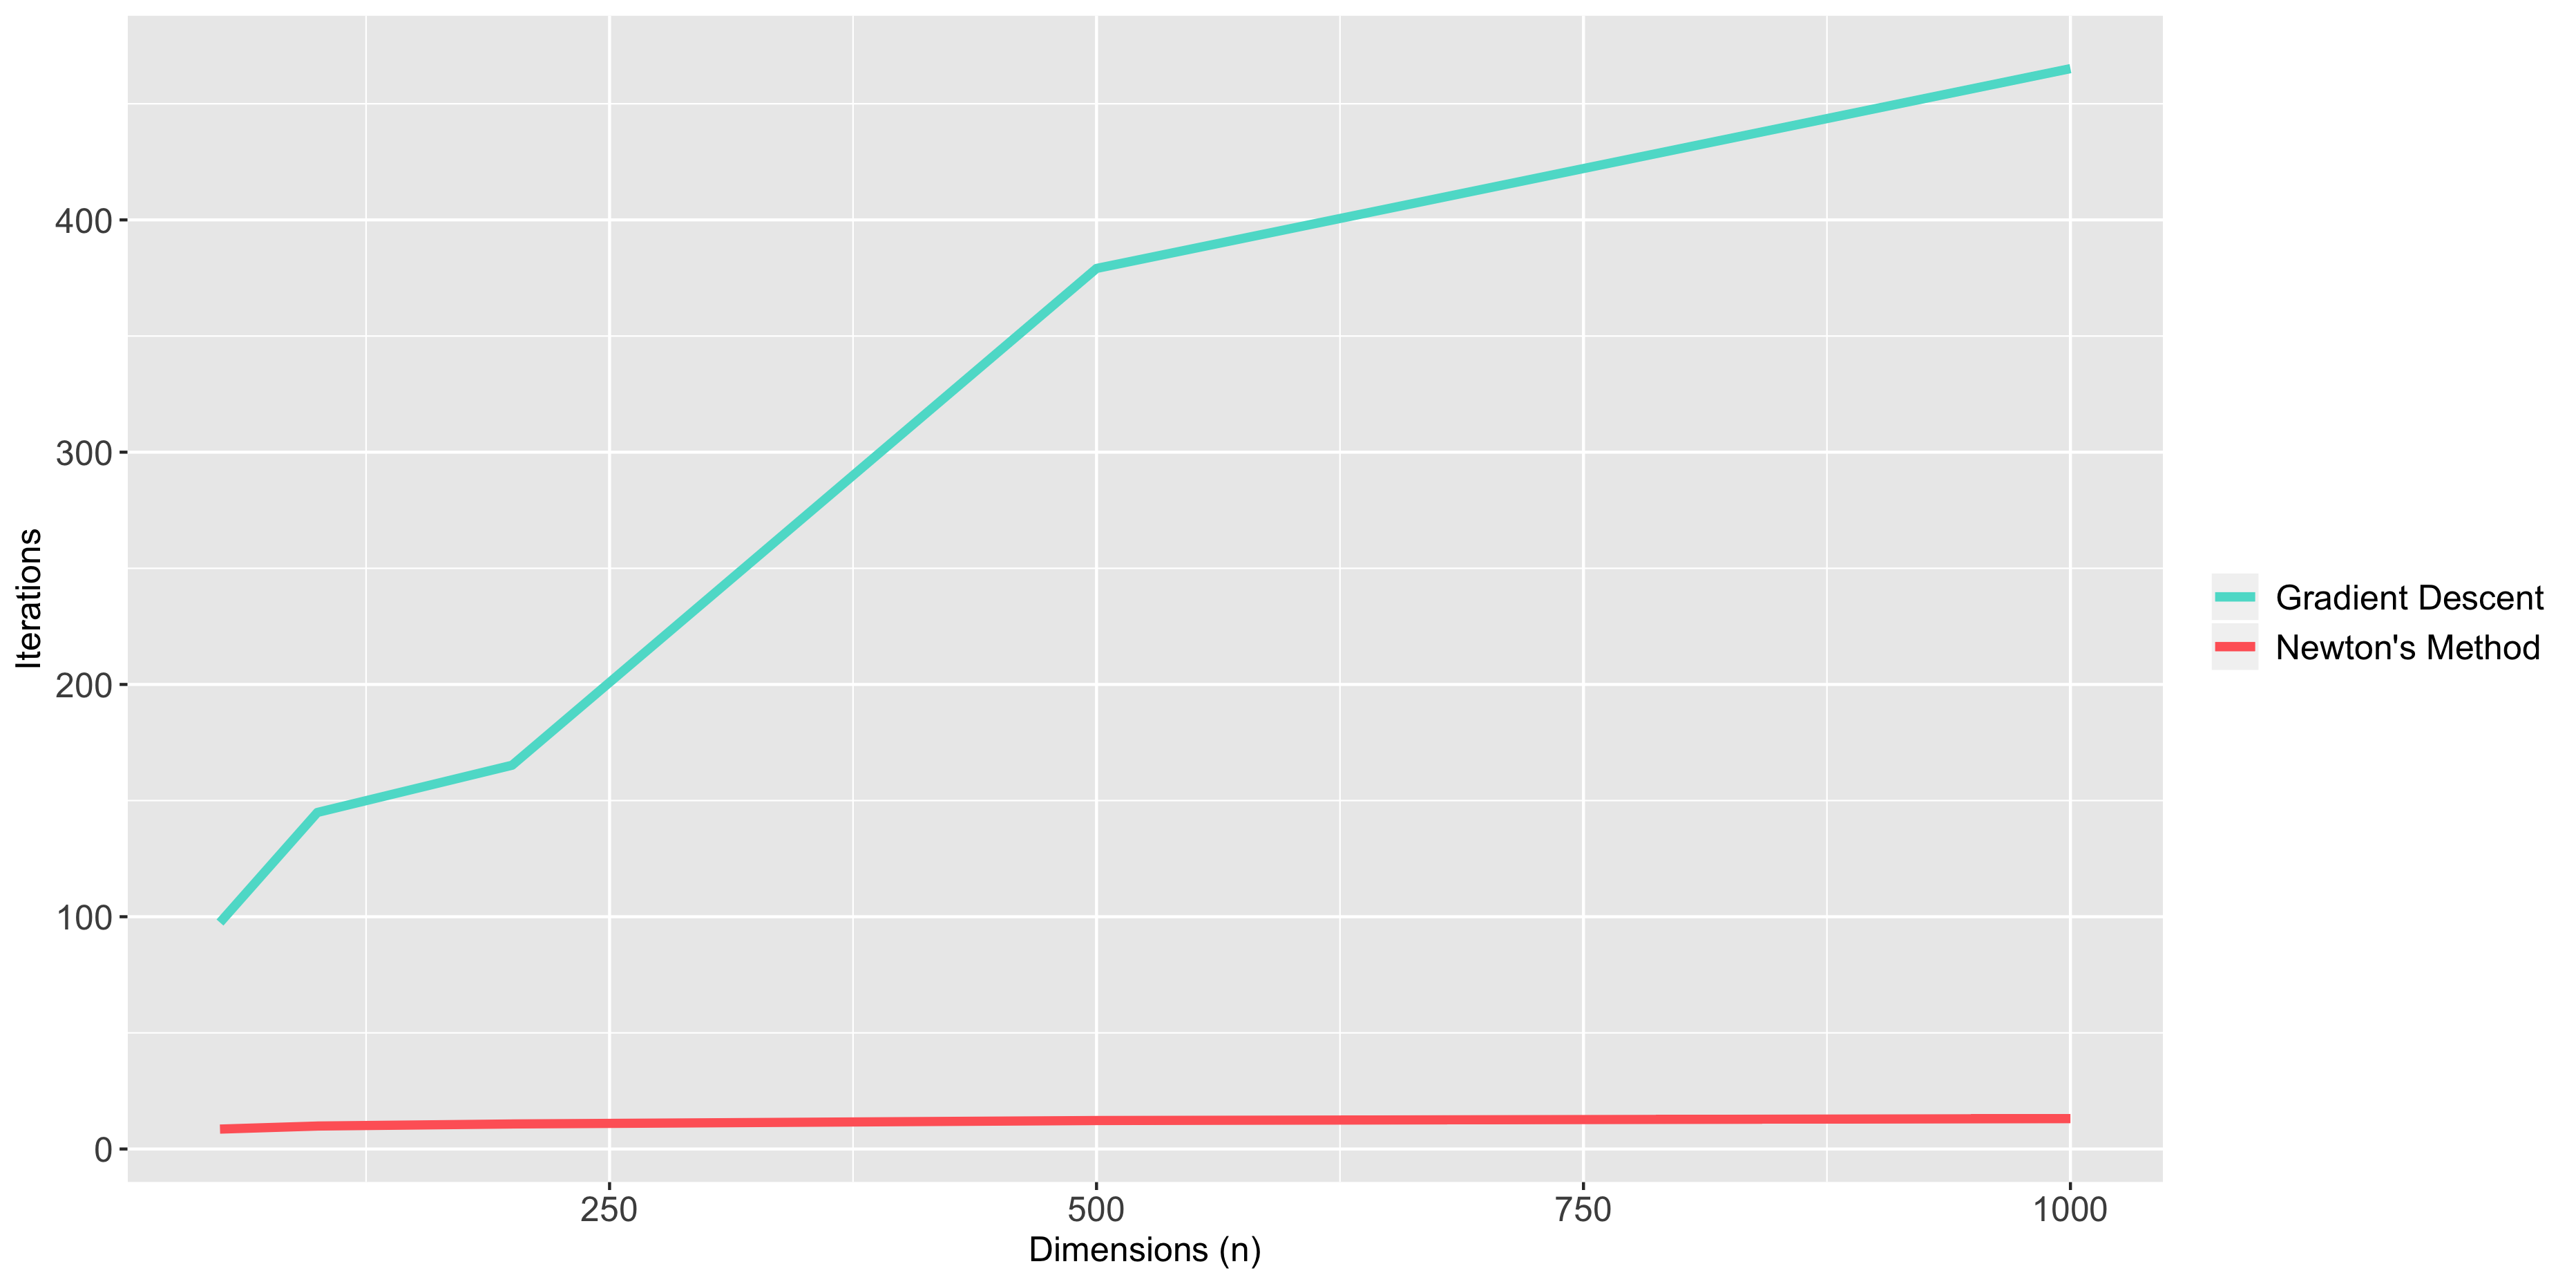
\includegraphics[clip, angle=0, width=13cm]{images/dimensions.png}
	\caption{Average number of iterations over dimensions ($n$)}
	\label{fig:dimensions}
	\floatfoot{Notes: The average number of iterations are calculated by averaging the number of iterations of 100 simulations for dimensions $n$ }
\end{figure}

\begin{table}[H]
	\centering
	\caption{Average number iterations over dimensions ($n$)}
	\label{dim_table}
	\begin{tabular}{llllll} \hline 
		\textbf{Dimensions} \cellcolor{gray!25} & \textbf{50} \cellcolor{gray!25} & \textbf{100} \cellcolor{gray!25} & \textbf{200} \cellcolor{gray!25} & \textbf{500} \cellcolor{gray!25} & \textbf{1000} \cellcolor{gray!25}  \\ \hline
		\textbf{Gradient Descent}  & 97.51 & 144.89 & 165.24 & 379.1 & 465.15 \\ \hline
		\textbf{Newton's Method} & 8.57 & 9.89 & 10.78 & 12.26 & 13.18 \\ \hline
	\end{tabular}
\end{table}

Nonetheless, when evaluating the average runtime of the algorithms over $n$ dimensions (see Figure \ref{fig:time} and Table \ref{time_table}), both methods show a similar pattern and do not differ considerably. In fact, at higher dimensions (i.e. $n = 500$ and $n = 1000$) gradient descent appears to be faster (on average). Thus, even though Newton's method requires fewer iterations, there are no differences in the runtime compared to gradient descent (if anything, Newton's method is slower at higher dimensions). This is likely due to the fact that Newton's method requires the Hessian to be derived and implemented, which requires $\mathcal{O}(n^2)$ operations and ”inverted” which requires $\mathcal{O}(n^3)$ operations. 

\begin{figure}[H]
	\centering
	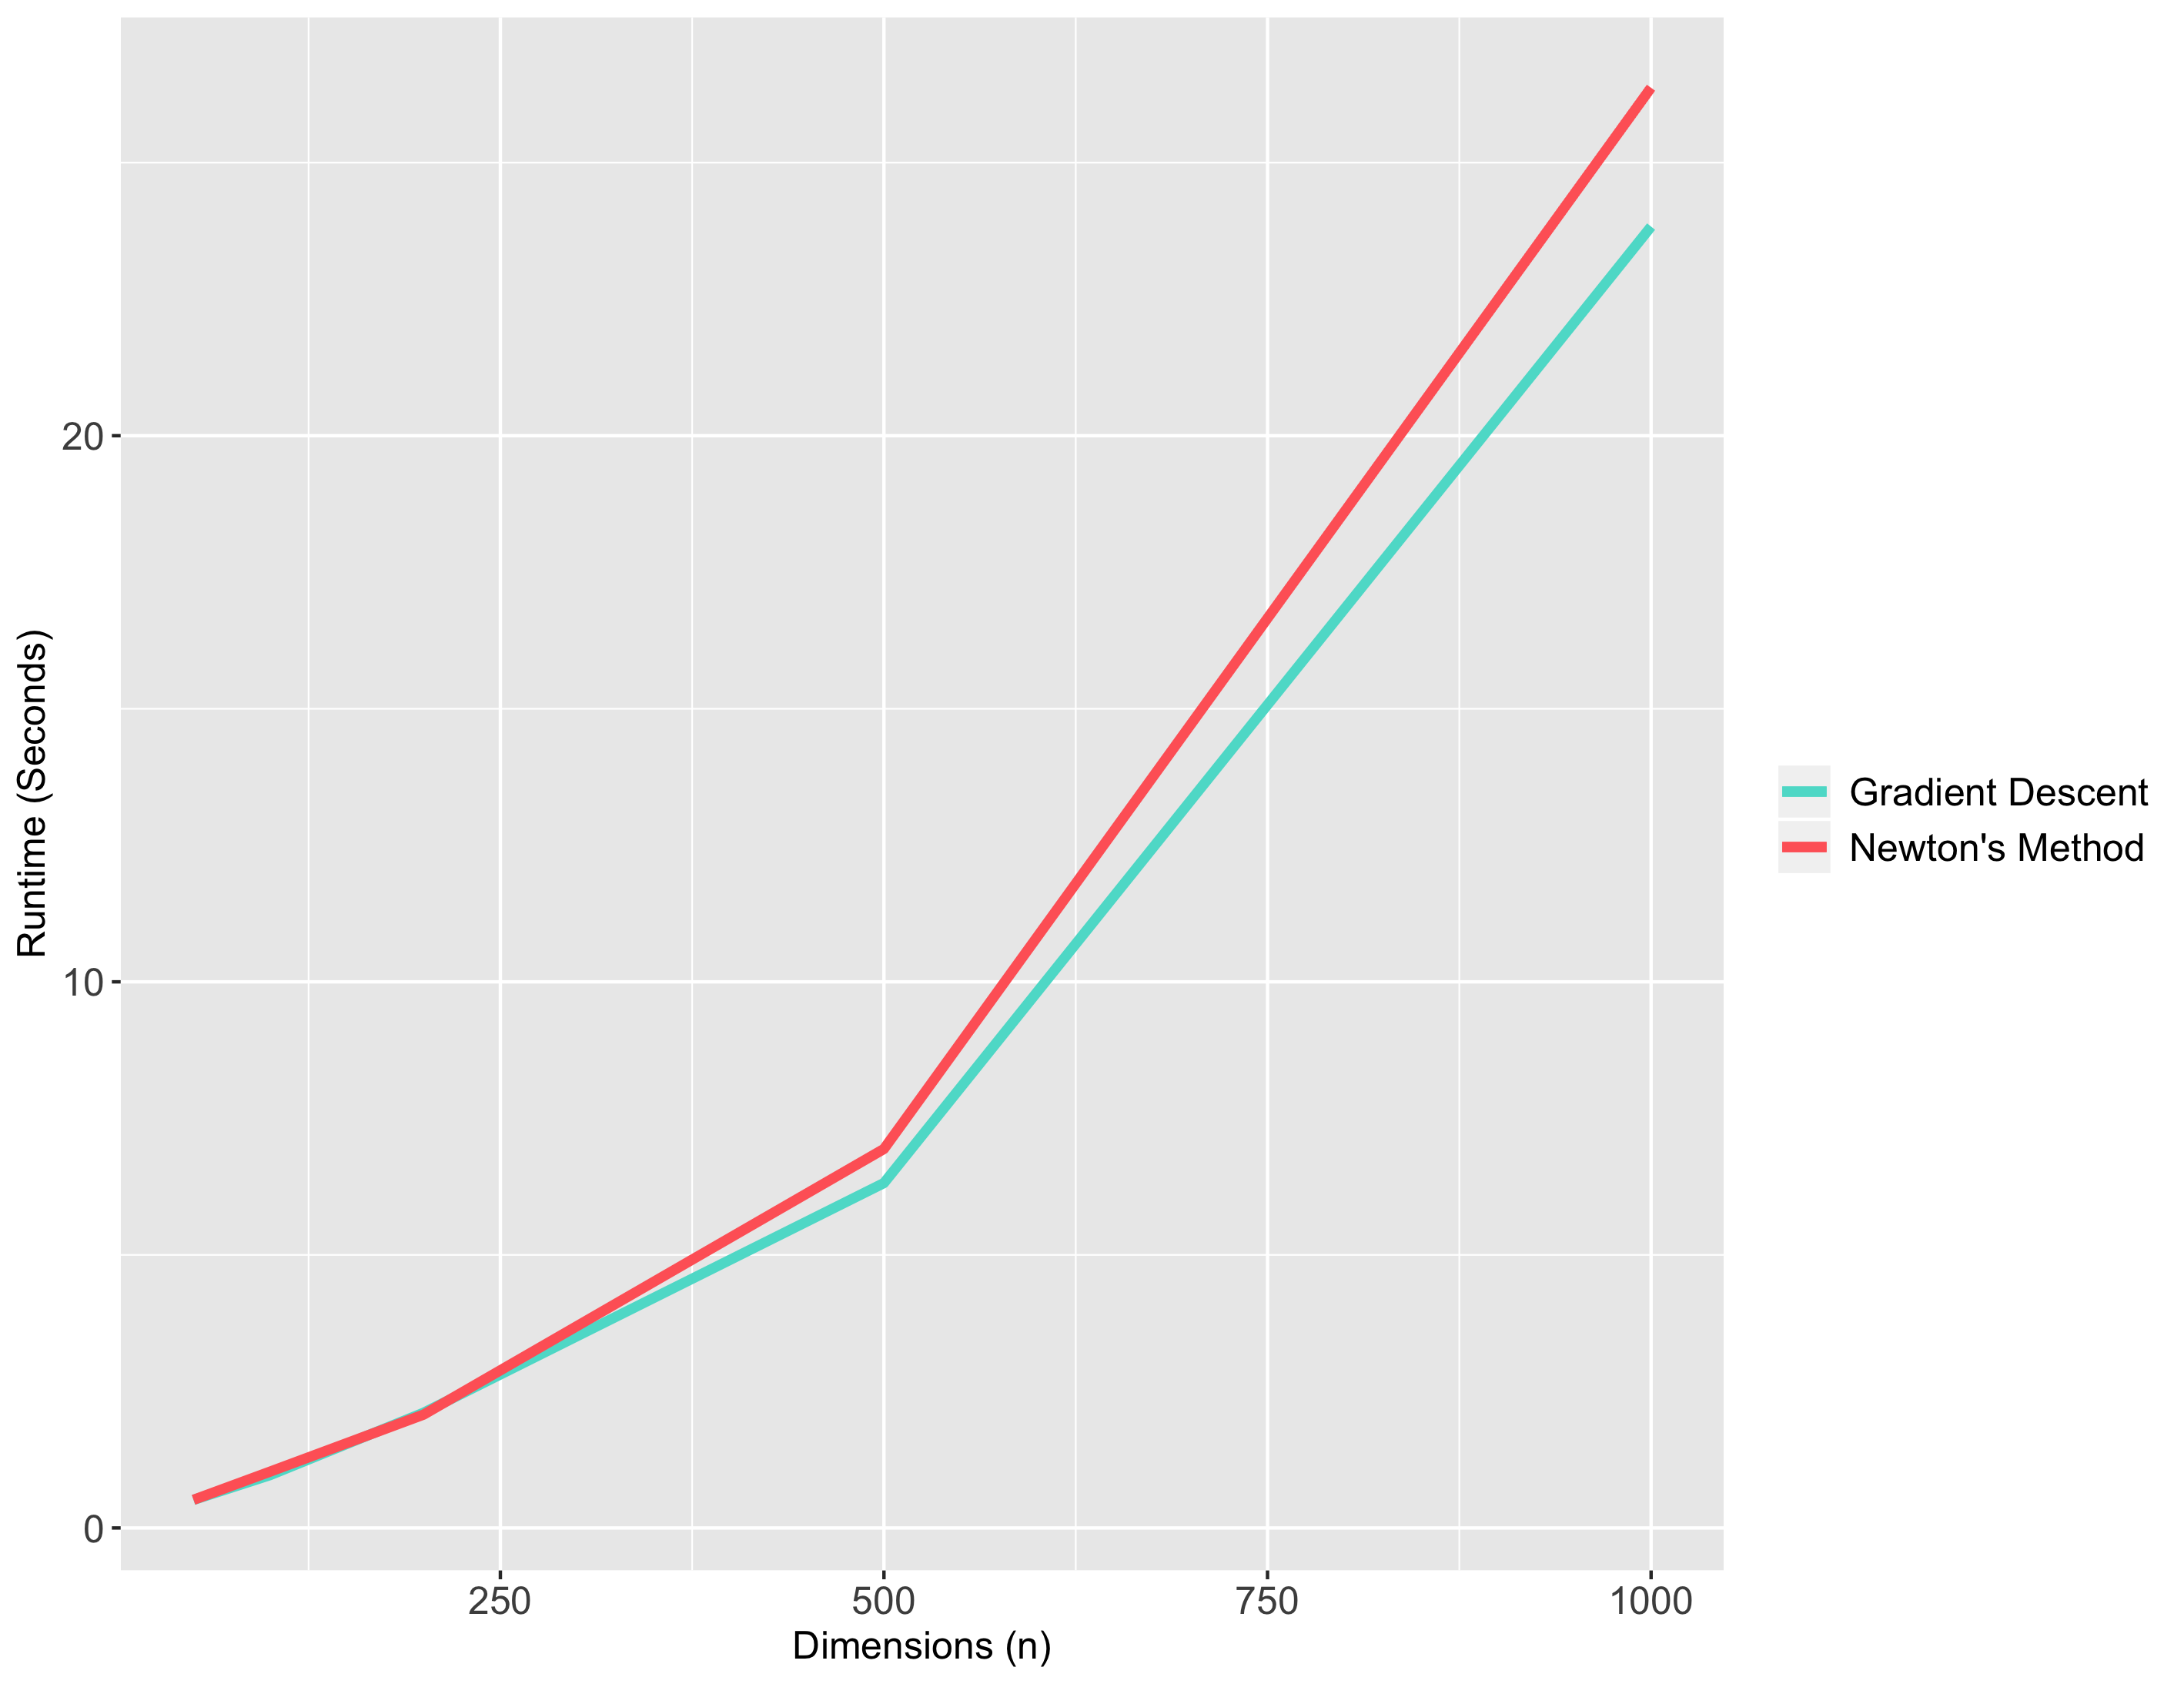
\includegraphics[clip, angle=0, width=13cm]{images/time.png}
	\caption{Average runtime (seconds) over dimensions ($n$)}
	\label{fig:time}
	\floatfoot{Notes: The average runtimes are calculated by averaging runtimes of 100 simulations for dimensions $n$ }
\end{figure}

\begin{table}[H]
	\centering
	\caption{Average runtime (seconds) over dimensions ($n$)}
	\label{time_table}
	\begin{tabular}{llllll} \hline
		\textbf{Dimensions} \cellcolor{gray!25} & \textbf{50} \cellcolor{gray!25} & \textbf{100} \cellcolor{gray!25} & \textbf{200} \cellcolor{gray!25} & \textbf{500} \cellcolor{gray!25} & \textbf{1000} \cellcolor{gray!25} \\ \hline
	\textbf{Gradient Descent}  & 0.51 & 0.97 & 2.11 & 6.32 & 23.83 \\ \hline
\textbf{Newton's Method}  & 0.52 & 1.03 & 2.08 & 6.94 & 26.37 \\ \hline
	\end{tabular}
\end{table}

%_______________________________________________________________________________________________________%
%BIBLIOGRAPHY
%_______________________________________________________________________________________________________%
%\pagebreak
%\bibliographystyle{agsm}
%\setcitestyle{authoryear}
%\bibliography{15D019.bib}

\appendix
\setcounter{figure}{0}

\end{document}
